\documentclass[11pt,a4paper]{article}
			\usepackage[french]{babel}
					
				\usepackage{pifont}  
				\usepackage[utf8x]{inputenc}
				\usepackage[T1]{fontenc} 
				\usepackage{lmodern}			
				\usepackage{fancyhdr}
				\usepackage{textcomp}
				\usepackage{makeidx}
				\usepackage{tabularx}
				\usepackage{multicol}
				\usepackage{multirow}
				\usepackage{longtable}
				\usepackage{color}
				\usepackage{soul}
				\usepackage{boxedminipage}
				\usepackage{shadow}
				\usepackage{framed}			
				\usepackage{array}
				\usepackage{url}
				\usepackage{ragged2e}
				\usepackage{fancybox}
				\newcommand{\cadretitre}[2]{
				  \vspace*{0.8\baselineskip}
				  \begin{center}%
				  \boxput*(0,1){%
					%\colorbox{white}{\Large\textbf{\ #1\ }}%
				  }%
				  {%
					\setlength{\fboxsep}{10pt}%
				    \Ovalbox{\begin{minipage}{.8\linewidth}\begin{center}\Large\sffamily{#2}\end{center}\end{minipage}}}%
				  \end{center}
				  \vspace*{2\baselineskip}
				  }
			
			\makeatletter
			\def\@seccntformat#1{\protect\makebox[0pt][r]{\csname the#1\endcsname\quad}}
			\makeatother

				% Permet d'afficher qqchose à une positin absolue
				\usepackage[absolute]{textpos}
				\setlength{\TPHorizModule}{1cm}
				\setlength{\TPVertModule}{\TPHorizModule}
	
				\usepackage[titles]{tocloft}
				\setlength{\cftbeforesecskip}{0.5ex}
				\setlength{\cftbeforesubsecskip}{0.2ex}
				\addto\captionsfrench{\renewcommand\contentsname{}}
				
				\usepackage[font=scriptsize]{caption}
				
				\usepackage{listings}
\lstdefinestyle{lstverb}
  {
    basicstyle=\footnotesize,
    frameround=tttt, frame=trbl, framerule=0pt, rulecolor=\color{gray},
    lineskip=-1pt,   % pour rapprocher les lignes
    flexiblecolumns, escapechar=\\,
    tabsize=4, extendedchars=true
  }
\lstnewenvironment{Java}[1][]{\lstset{style=lstverb,language=java,#1}}{}
				\ifx\pdfoutput\undefined
					\usepackage{graphicx}
				\else
					\usepackage[pdftex]{graphicx}
				\fi
				\usepackage[a4paper, hyperfigures=true, colorlinks, linkcolor=black, citecolor=blue,urlcolor=blue, pagebackref=true, bookmarks=true, bookmarksopen=true,bookmarksnumbered=true,
                pdfauthor={}, pdftitle={TD Packages}, pdfkeywords={TD Packages, },pdfpagemode=UseOutlines,pdfpagetransition=Dissolve,nesting=true,
				backref, pdffitwindow=true, bookmarksnumbered=true]{hyperref}
				\usepackage{supertabular}
				\usepackage[table]{xcolor}
				\usepackage{url}
				\usepackage{caption} 
				\setlength{\parskip}{1.3ex plus 0.2ex minus 0.2ex}
				\setlength{\parindent}{0pt}
				
				\makeatletter
				\def\url@leostyle{ \@ifundefined{selectfont}{\def\UrlFont{\sf}}{\def\UrlFont{\footnotesize\ttfamily}}}
				\makeatother
				\urlstyle{leo}
				
				\definecolor{examplecolor}{rgb}{0.156,0.333,0.443}
				\definecolor{definitioncolor}{rgb}{0.709,0.784,0.454}
				\definecolor{exercisecolor}{rgb}{0.49,0.639,0}
				\definecolor{hintcolor}{rgb}{0.941,0.674,0.196}
				\definecolor{tableHeadercolor}{rgb}{0.709,0.784,0.454}
				\definecolor{tablerowAltcolor}{rgb}{.866,.905,.737}
				\definecolor{tablerowAlt2color}{rgb}{.968,.976,.933}
				\definecolor{verylightgray}{rgb}{0.98,0.98,0.98}
				
				\newenvironment{fshaded}{
				\def\FrameCommand{\fcolorbox{framecolor}{shadecolor}}
				\MakeFramed {\FrameRestore}}
				{\endMakeFramed}
				
				\newenvironment{fexample}[1][]{\definecolor{shadecolor}{rgb}{.913,.913,.913}
				\definecolor{framecolor}{rgb}{.156,.333,.443}
				\begin{fshaded}}{\end{fshaded}} 
				
				\newenvironment{fdefinition}{\definecolor{shadecolor}{rgb}{.913,.913,.913}
				\definecolor{framecolor}{rgb}{.709,.784,.454}
				\begin{fshaded}}{\end{fshaded}}
				
				\newenvironment{fexercise}{\definecolor{shadecolor}{rgb}{.913,.913,.913}
				\definecolor{framecolor}{rgb}{.49,.639,0}
				\begin{fshaded}}{\end{fshaded}}
				
				\newenvironment{fhint}{\definecolor{shadecolor}{rgb}{.913,.913,.913}
				\definecolor{framecolor}{rgb}{.941,.674,.196}
				\begin{fshaded}}{\end{fshaded}}	
				
				\newcommand{\PreserveBackslash}[1]{
				\let\temp=\\#1\let\\=\temp
				}
				\let\PBS=\PreserveBackslash
				\newcolumntype{A}{>{\PBS\raggedright\small\hspace{0pt}}X}
				\newcolumntype{L}[1]{>{\PBS\raggedright\small\hspace{0pt}}p{#1}}
				\newcolumntype{R}[1]{>{\PBS\raggedleft\small\hspace{0pt}}p{#1}}
				\newcolumntype{C}[1]{>{\PBS\centering\small\hspace{0pt}}p{#1}}
				
				\makeindex
				
				\title{TD Packages}	
			\date{}
			\author{\scriptsize{}}
			\definecolor{light-gray}{gray}{0.8}
			\renewcommand{\headrulewidth}{0pt}
			\fancyhead[L]{
				\footnotesize\textsc{Haute \'Ecole de Bruxelles}\\
	    			\footnotesize\textsc{\'Ecole Sup\'erieure d'Informatique}
			}
			\fancyhead[R]{
				\footnotesize{Bachelor en Informatique}\\
				\footnotesize{Laboratoires Java} - 
			\footnotesize{1\`ere ann\'ee}}
				\fancyfoot[L]{ }
				\fancyfoot[C]{}
				\fancyfoot[R]{\scriptsize{\textcolor{gray}{version 2014-2015 (\today)}}}
				\pagestyle{plain}
				\reversemarginpar
				\usepackage{rotating}						
				\begin{document}
					\begin{textblock}{9}(2,3.2)
						
\includegraphics[width=2cm]{../../../_templates/java/icons/logo-esi}
					\end{textblock}
				
				
				
				
				%\maketitle
				\cadretitre{TD1}{TD Packages}
				\thispagestyle{fancy}
        \marginpar{\begin{sideways}
            \begin{minipage}[t]{1cm}
            \begin{tiny}
            
\includegraphics[width=1\linewidth,height=1\textheight,keepaspectratio=true]{../../../_templates/java/icons/cc-gris.jpg}
			\end{tiny}
			\end{minipage}
            \begin{minipage}[b]{19cm}
            \begin{tiny}
            \textcolor{gray}{Distribué sous licence Creative Commons Paternité - Partage à l'Identique 2.0 Belgique 
            (\texttt{http://creativecommons.org/licenses/by-sa/2.0/be/})
			\vspace{-1em}
			\\Les autorisations au-delà du champ de cette licence peuvent être obtenues à 
			\texttt{http://www.heb.be/esi}
			- \texttt{mcodutti@heb.be}
			}\end{tiny}
			\end{minipage}
        \end{sideways}}
            \begin{abstract}
			Ce TD a pour but d'aborder comment associer un package \`a vos m\'ethodes.
		
            \par
        \end{abstract}
				\vspace{-2em}\tableofcontents
				\pagestyle{plain}
            \clearpage
            \fancyhead[L,C,R]{}
            \fancyfoot[L,C]{}
            \fancyfoot[R]{ \scriptsize{\textcolor{gray}{
				TDPackage - page \thepage}}}
				\thispagestyle{fancy}
				\pagestyle{fancy}
	   
            \section{Les package}\subsection{Introduction aux packages}
				Vous \^etes capables d'utiliser une classe
				qui a \'et\'e plac\'ee dans un package standard 
				(comme \verb@java.util.Scanner@).
				Nous allons \`a pr\'esent vous montrer
				comment placer vos propres classes dans des packages
				et les utiliser.
			
            \par
        
			
		\subparagraph{Le nom d'un package} 
		
					\textcolor{white}{.} \par
				
            \par
        
				Un nom de package doit \^etre choisi de telle sorte
				\`a repr\'esenter l'organisation \`a laquelle elle
				appartient et le projet associ\'e ou
				le type de classe.
				Il ne faut pas se baser sur l'endroit o\`u sont plac\'es 
				les fichiers sources.
			
            \par
        
				Pour \textbf{votre} code, 
				nous vous recommandons de rassembler vos classes
				par package reprenant votre login et le TD.
				Exemple : \verb|g32010.tdPackage|. 
			
            \par
        
			
		\subparagraph{Associer une classe \`a un package} 
		
					\textcolor{white}{.} \par
				
            \par
        
				L'appartenance d'une classe \`a un package d\'etermin\'e est n\'ecessaire \`a la compilation. 
				D\`es lors vous devrez ajouter comme \textbf{premi\`ere instruction du source} 
				(c-\`a-d avant m\^eme l'instruction \verb|public class NomClasse|) :
			
            \par
        \begin{Java}
	package g32010.tdPackage;
			\end{Java}
			
		\subparagraph{Nom complet d'une classe} 
		
					\textcolor{white}{.} \par
				
            \par
        
				Le nom 
				\textbf{qualifi\'e} 
				d'une classe 
				(on dit aussi \textbf{nom complet})
				est obtenu en accolant
				le nom de la classe au nom du package ;
				on obtient ainsi un nom unique pour cette classe.
				C'est ce nom qu'il faudra utiliser pour 
				\textbf{ex\'ecuter} la classe.
			
            \par
        
				Par exemple, le nom complet de la classe \verb@Color@ 
				dont le package est \verb|esi.util|
				est \verb|esi.util.Color|. 
			
            \par
        
						Donnez le nom complet de la classe \verb@SurfaceTriangle@
						dont le package est \verb@g32010.tdPackage@ :
					 \textcolor{gray}{\underline{\hspace*{20em}}} 
			
		\subparagraph{Package et dossiers} 
		
					\textcolor{white}{.} \par
				
            \par
        
				Alors qu'on peut placer ses fichiers sources (les .java)
				o\`u on veut, ce n'est pas le cas pour les fichiers
				compil\'es (les .class) d\`es lors qu'on joue avec des packages.
				Ils devront \^etre plac\'es \`a un endroit bien pr\'ecis
				pour que le compilateur et la machine virtuelle
				puissent les retrouver.
			
            \par
        			
				La notion de package est li\'ee \`a celle de r\'epertoire
				(et m\^eme d'arborescence de r\'epertoires).
				Ainsi le package
				\verb|td.tdPackage| sera associ\'e 
				aux dossiers \verb@td/tdPackage@
				(un dossier \verb|tdPackage| 
				dans un dossier \verb|td|).
				Tout comme une classe appartient \`a un package,
				la version compil\'ee de la classe
				devra se trouver dans les dossiers correspondant au package.
			
            \par
        
			
		\subparagraph{Exemple} 
		
					\textcolor{white}{.} \par
				
            \par
        
				Si \verb|Color| 
				a pour package \verb|esi.util|,
				le fichier \verb@Color.class@
				devra se trouver dans le r\'epertoire associ\'e 
				\verb@esi/util@.
			
            \par
        
			
		\subparagraph{Exercice} 
		
					\textcolor{white}{.} \par
				
            \par
        
				Examinez le contenu du dossier 
				\verb@esi/util@
				qui se trouve dans 
				\verb@/eCours/Java@.
			
            \par
        
			
		\subparagraph{Exercice} 
		
                \textcolor{white}{.} \par
            
						Donnez la suite de r\'epertoires dans lesquels 
						\textbf{doit} certainement
						se trouver la classe \verb|SurfaceTriangle|
						dont le package est \verb|g32010.tds.tdPackage| \textcolor{gray}{\underline{\hspace*{16em}}} \subsection{Utiliser le package d'un autre}
			Une classe
			\verb@Color@
			a comme package
			\verb@esi.util@.
			Voyons comment l'utiliser.			
		
            \par
        
			
		\subparagraph{Exp\'erience} 
		
					\textcolor{white}{.} \par
				
            \par
        
					\begin{enumerate}
				
			\item 
				La classe poss\`ede une m\'ethode principale.
				Tentez de l'ex\'ecuter via la commande
				\verb@java Color@.
				\par
				
				Ca ne fonctionne pas. Pourquoi ?
			
			\item 
				Mais bien s\^ur ; on a dit qu'il fallait utiliser
				le nom complet de la classe.
				Tentez la commande
				\verb@java esi.util.Color@.
				\par
				
				Zut ! Ca ne fonctionne toujours pas. Pourquoi ?
			
			\item 
					Parce que Java ne sait pas o\`u trouver la classe
					et il est hors de question de chercher dans
					tout le syst\`eme de fichier.
				
            \par
        
					O\`u est-elle d'ailleurs, cette classe ?
				
            \par
        
					Lan\c cez la commande
					\verb@find /eCours/java -name Color.class@
					pour le savoir.
					Vous devriez voir que la classe se trouve exactement ici :
					\verb@/eCours/java/esi/util/Color.class@
            \par
        
			\item 
				On va indiquer \`a Java o\`u chercher.
				Entrez la commande
				\par
				\verb@java -cp /eCours/java esi.util.Color@.
				\par
				
				Cette fois-ci \c ca fonctionne !
			
					\end{enumerate}
				
			L'option \verb@cp@
			(une abr\'eviation pour \verb@classpath@)
			indique le (ou les) endroit(s) o\`u chercher les classes.
		
            \par
        \textbf{Important ! }
			on ne donne pas le dossier o\`u se trouve le
			\textit{.class}
			mais le dossier o\`u il va pouvoir trouver
			la hi\'erarchie de dossiers li\'ee au package.
			Finalement, le fichier se trouve \`a un endroit
			qui est la \textit{concat\'enation}
			de l'option \textit{cp}
			et du package.
		
            \par
        \subsection{Utiliser ses propres packages}
			\`A pr\'esent, 
			nous allons voir comment vous pouvez placer
			vos propres classes dans un package.
		
            \par
        
			
		\subparagraph{Exp\'erience} 
		
					\textcolor{white}{.} \par
				
            \par
        
					\begin{enumerate}
				
			\item 
				Prenez une copie de la classe 
				\verb@Color@.	
			
			\item 
				Ajoutez comme premi\`ere ligne :
				\begin{Java}
	package g12345.util;
				\end{Java}
			\item 
				Compilez-la : \verb@javac Color.java@.
			
			\item 
				Ex\'ecutez-la : \verb@java -cp . g12345.util.Color@.
				\par
				
				\c Ca ne fonctionne pas ! Pourquoi ?
			
			\item 
				Qu'on est b\^ete !
				Java cherche le fichier dans une hi\'erarchie
				de dossiers correspondant au package.
				Ici, il cherche le fichier
				\verb@g12345/util/Color.class@
			\item 
				D\'epla\c cons le fichier au bon endroit.
				\par
				\verb@mkdir -p g12345/util@\par
				\verb@mv Color.class g12345/util@
			\item 
				Re-tentons : \verb@java -cp . g12345.util.Color@.
				\par
				
				\c Ca fonctionne !
			
					\end{enumerate}
				
			
		\subparagraph{J'ai oubli\'e l'option '-cp' et \c ca fonctionne quand m\^eme !?} 
		
					\textcolor{white}{.} \par
				
            \par
        
			En effet, sur linux1, et nous verrons pourquoi,
			si on ne lui  dit pas o\`u chercher, 
			il cherche dans le dossier courant.
		
            \par
        
			
		\subparagraph{L'option -d} 
		
					\textcolor{white}{.} \par
				
            \par
        
			Ce serait p\'enible de devoir d\'eplacer,
			apr\`es chaque compilation,
			la classe au bon endroit.
			Heureusement, le compilateur propose une option
			qui place directement le fichier g\'en\'er\'e au bon endroit.
		
            \par
        
			La commande
		
            \par
        \begin{Java}
	java -d chemin Fichier.java
		\end{Java}
			compile le fichier donn\'e et place
			le r\'esultat dans une hi\'erarchie de dossiers
			qui correspond au package \`a partir du chemin donn\'e.
		
            \par
        
			
		\subparagraph{Exemple} 
		
					\textcolor{white}{.} \par
				
			Pour la classe couleur, 
			on aurait pu compiler simplement avec la commande :
			\verb@javac -d . Color.java@
			pour indiquer de cr\'eer le r\'esultat dans le dossier
			\verb@./g12345/util/@.
		
            \par
        \subsection{La variable CLASSPATH}
				Sp\'ecifier \`a chaque fois,
				l'option \verb@cp@
				est p\'enible.
				Ce serait bien de pouvoir lui dire une fois pour toutes
				o\`u chercher.
				C'est exactement le r\^ole de la variable d'environnement
				\verb@CLASSPATH@.
			
            \par
        
			\begin{boxedminipage}[h]{\linewidth}
		
				La variable
				\verb@CLASSPATH@
				contient une liste de dossiers o\`u chercher les
				classes. Chaque dossier est s\'epar\'e par 
				"\verb@:@".
			
			\end{boxedminipage}

				Pour la manipuler,
				la proc\'edure est la m\^eme que pour les
				autres variables d'environnement.
			
            \par
        
					\begin{itemize}
				
			\item 
					Pour voir son contenu : 
					\verb@echo $CLASSPATH@
			\item 
					Pour changer son contenu : 
					\verb@CLASSPATH=valeur@
			\item 
					Pour ajouter un dossier \`a son contenu : 
					\verb@CLASSPATH=$CLASSPATH:valeur@
			\item 
					Si elle est d\'efinie pour la premi\`ere fois : 
					\verb@export CLASSPATH@
			\item 
					Si la modification doit \^etre permanente,
					vous pouvez placer la commande dans le fichier
					\verb@.bashrc@
					\end{itemize}
				
			
		\subparagraph{Exercice} 
		
					\textcolor{white}{.} \par
				
				Affichez le contenu actuel 
				de la variable 
				\verb@CLASSPATH@.
				Que signifie le "." ?
			
            \par
        
			
		\subparagraph{Exercice} 
		
                \textcolor{white}{.} \par
            
						Sachant que la classe \verb|SurfaceTriangle| se trouve dans 
						\verb@/home/g32010/tds/tdPackage@ 
						et qu'on retrouve \verb@/home@ dans la variable \verb@CLASSPATH@, 
						donnez l'instruction \verb|package| correspondant \`a la situation :
					\begin{Java}
package  \\_\\_\\_\\_\\_\\_\\_\\_\\_\\_\\_\\_\\_\\_\\_\\_\\_\\_\\_\\_\\_\\_\\_\\_\\_\\_\\_ ;
						\end{Java}
			
		\subparagraph{Exercice} 
		
                \textcolor{white}{.} \par
            
						Supposons que la classe \verb|Exercice1|
						a pour package \verb|esi.lg1.exemples|
						et qu'elle a comme chemin 
						\verb@/eCours/java/be/heb/esi/lg1/exemples/Exercice1.class@, 
						donnez la hi\'erarchie de r\'epertoires \`a ajouter au \verb@CLASSPATH@.
					
						CLASSPATH=\$CLASSPATH: \textcolor{gray}{\underline{\hspace*{16em}}} 
			
		\subparagraph{Exercice} 
		
					\textcolor{white}{.} \par
				
				Faites ce qu'il faut pour pouvoir
				ex\'ecuter \textbf{notre}
				classe \verb@Color@
				(package \verb@esi.util@)
				sans utiliser l'option \verb@-cp@.
			
            \par
        \subsection{Organiser ses fichiers}
				R\'esumons ce que  nous avons d\'ej\`a vu.
			
            \par
        
					\begin{itemize}
				
			\item 
					un package est un regroupement de classes ;
				
			\item 
					pour cr\'eer un tel package,
					il suffit de commencer les 
					\textbf{fichiers sources} 
					contenant les classes \`a regrouper
					par l'instruction 
					\verb@package@ 
					suivi du nom 
					que l'on d\'esire donner au package ;
				
			\item 
					les \textbf{fichiers classes} 
					doivent se trouver dans l'arborescence de r\'epertoires 
					donn\'ee par le package.
				
			\item 
					Cette arborescence doit commencer dans un dossier
					repris dans le CLASSPATH.
				
					\end{itemize}
				
				Mais, concr\'etement,
				quel dossier choisir pour placer les classes ?
				Il existe plusieurs fa\c cons de s'organiser ;
				on va vous en pr\'esenter deux. 
			
            \par
        
			
		\subparagraph{Sans package.} 
		
					\textcolor{white}{.} \par
				
				D'abord, r\'esumons ce que vous faisiez jusqu'\`a pr\'esent
				sans package.
				Avec cette approche, le source et la classe
				se trouvent dans un m\^eme dossier, quelconque.
			
            \par
        
					\begin{enumerate}
				
			\item 
					On se place o\`u on veut.
				
			\item 
					On \'edite le source : \verb@nano Test.java@
			\item 
					On compile : \verb@javac Test.java@
			\item 
					On ex\'ecute : \verb@java Test@
					\end{enumerate}
				
			
		\subparagraph{1re proposition : pour transporter vos sources et classes rapidement.} 
		
					\textcolor{white}{.} \par
				
            \par
        
				Dans cette approche, les sources sont s\'epar\'es des classes
				mais sont dans un dossier commun.
			
            \par
        \begin{figure}[hbt]
				    \begin{center}
					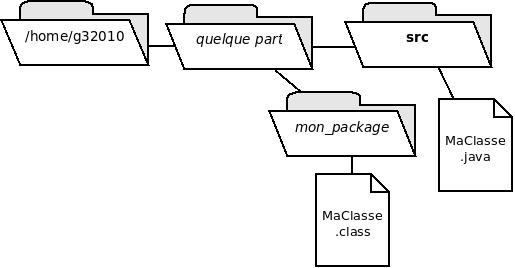
\includegraphics[width=0.6\linewidth,height=0.8\textheight,keepaspectratio=true]{/home/clr/Documents/Cours/DEV1Q2/TDPackage/fr/image/approche4.jpeg}
						\end{center}
                
                    \caption[Illustration de la 1\`ere approche]{Illustration de la 1\`ere approche}
                \end{figure}
                    
					\begin{enumerate}
				
			\item 
					On v\'erifie que le CLASSPATH contient bien le 
					dossier courant (sur linux1, c'est le cas).
				
			\item 
					On se place quelque part.
				
			\item 
					On cr\'ee un dossier pour les sources : \verb@mkdir src@
			\item 
					On \'edite le source dans le dossier d\'edi\'e : 
					\par
				\verb@nano src/Test.java@\par
				
					en prenant soin de commencer le fichier par un package qui a du sens
					(par exemple : \verb@g12345.tdPackage@).
				
			\item 
					On compile en demandant \`a cr\'eer la classe \`a partir
					du dossier courant : 
					\par
				\verb@javac -d . src/Test.java@
			\item 
					On ex\'ecute : \verb@java g12345.tdPackage.Test@
					\end{enumerate}
				
			
		\subparagraph{Exercice} 
		
					\textcolor{white}{.} \par
				
            \par
        
				Dans un sous-dossier du tdPackage
				(par exemple : tdPackage/cas1),
				faites une copie de votre programme 
				\verb@Hello.java@
				et placez-le dans un package en suivant
				l'approche ci-dessus.
				Quelle est la commande \`a utiliser pour compiler ?
				Et pour ex\'ecuter ?
			
            \par
        
			\fcolorbox{gray}{verylightgray}{
			\begin{minipage}[c][2cm][c]{\textwidth}\textcolor{verylightgray}{X}\end{minipage}
		}\par\medskip
			
		\subparagraph{Remarques} 
		
					\textcolor{white}{.} \par
				
            \par
        
					\begin{enumerate}
				
			\item 
					Il existe de nombreuses variantes.
					Par exemple, les sources dans le dossier
					"src" et les classes dans le dossier "classes"
					ou encore les classes dans le dossier "classes"
					mais les sources directement dans le dossier
					courant. 
				
			\item 
					Cette approche permet de facilement
					copier tous les sources et les classes associ\'ees
				
			\item 
					Par contre, les classes ne peuvent pas s'ex\'ecuter
					de partout.
			 	
					\end{enumerate}
				
			
		\subparagraph{2e proposition : toutes les classes sont regroup\'ees dans le m\^eme dossier (\char`\~/classes).} 
		
					\textcolor{white}{.} \par
				
            \par
        
				Dans cette approche, toutes les classes
				de tous vos projets sont plac\'ees dans un dossier commun
				(par exemple : \verb@~/classes@)
			
            \par
        \begin{figure}[hbt]
				    \begin{center}
					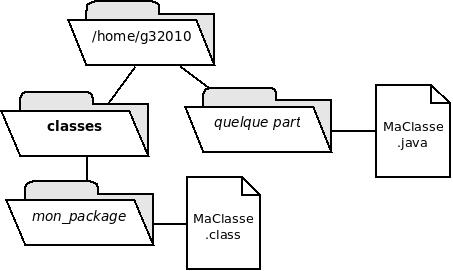
\includegraphics[width=0.6\linewidth,height=0.8\textheight,keepaspectratio=true]{/home/clr/Documents/Cours/DEV1Q2/TDPackage/fr/image/approche3.jpeg}
						\end{center}
                
                    \caption[Illustration de la 2\`eme approche]{Illustration de la 2\`eme approche}
                \end{figure}
                    
					\begin{enumerate}
				
			\item 
					Il faut s'assurer que le CLASSPATH contienne 
					le dossier \verb@~/classes@.
					Si ce n'est pas le cas,
					il faut le d\'efinir (une fois pour toutes
					dans le fichier de configuration du bash) :
					\verb@CLASSPATH=$CLASSPATH:~/classes@.					
				
			\item 
					On se place quelque part.
				
			\item 
					On \'edite le source directement dans le dossier courant : 
					\verb@nano Test.java@
					en prenant soin de commencer le fichier par un package qui a du sens
					(par exemple : \verb@g12345.tdPackage@).
				
			\item 
					On compile en demandant \`a cr\'eer la classe dans
					le dossier global d\'edi\'e :
					\verb@javac -d ~/classes Test.java@
			\item 
					On ex\'ecute : \verb@java g12345.tdPackage.Test@
					\end{enumerate}
				
			
		\subparagraph{Exercice} 
		
					\textcolor{white}{.} \par
				
            \par
        
				Il s'agit du m\^eme exercice que pour la premi\`ere approche.
				Dans un autre sous-dossier du tdPackage
				(par exemple : tdPackage/cas2),
				faites une copie de votre programme 
				\verb@Hello.java@
				et placez-le dans un package en suivant
				l'approche ci-dessus.
				Quelle est la commande \`a utiliser pour compiler ?
				Et pour ex\'ecuter ?
			
            \par
        
			\fcolorbox{gray}{verylightgray}{
			\begin{minipage}[c][2cm][c]{\textwidth}\textcolor{verylightgray}{X}\end{minipage}
		}\par\medskip\section{Exercices}
				Maintenant, mettons tout \c ca en pratique.
      
            \par
        \subsection{La notion de package}
			
		\subparagraph{API} 
		
                \textcolor{white}{.} \par
            
								Ouvrez la documentation de l'API Java 
								et recherchez la classe qui se nomme
								\verb@IllegalFormatException@.
							
            \par
        
					\begin{itemize}
				
			\item 
									Quel est le package de cette classe ?   
									 \textcolor{gray}{\underline{\hspace*{10em}}} 
			\item 
									Quel est le nom qualifi\'e de cette classe ?\par
				 \textcolor{gray}{\underline{\hspace*{20em}}} 
					\end{itemize}
				
								\'Ecrivez la d\'eclaration correcte d'une variable nomm\'ee
								\verb@clavier@ de type 
								\verb@Scanner@ sans import de la classe.
							
            \par
         \textcolor{gray}{\underline{\hspace*{16em}}}  \textcolor{gray}{\underline{\hspace*{5em}}} 
            \par
        
			
		\subparagraph{Choix Multiple } 
		
                \textcolor{white}{.} \par
            Soit le code :
            \par
        \begin{Java}
package td.tdPackage; 
public class ErrCompilation {
    import java.util.Scanner;
    public static void main (String [] args) { 
        System.out.println("TDPackage");
    }
}							\end{Java}
								la commande \verb@javac ErrCompilation.java@ 
								provoque les erreurs suivantes :
							
            \par
        \begin{scriptsize}\begin{verbatim}
ErrCompilation.java:2: illegal start of type
import java.util.Scanner;
^
ErrCompilation.java:2: ';' expected
import java.util.Scanner;
^
ErrCompilation.java:2: illegal start of type
import java.util.Scanner;
^
ErrCompilation.java:2: ';' expected
import java.util.Scanner;
^
ErrCompilation.java:2: <identifier> expected
import java.util.Scanner;
^
5 errors
							\end{verbatim}\end{scriptsize}
							Il s'agit d'erreurs g\'en\'er\'ees par le compilateur car :
							
            \par
        
            \begin{itemize} 
        
            \item[ \ding{"6D} ] \verb|import| s'\'ecrit avec une majuscule
        
            \item[ \ding{"6D} ] le package utilis\'e est incorrect
        
            \item[ \ding{"6D} ] le \verb|import| est mal plac\'e dans le code
        
            \item[ \ding{"6D} ] \verb|Scanner| s'\'ecrit avec une minuscule
        
            \item[ \ding{"6D} ] on n'utilise pas \verb|Scanner| dans le code
        
            \end{itemize} 
        
			
		\subparagraph{Choix Multiple } 
		
                \textcolor{white}{.} \par
            Soit le code :
            \par
        \begin{Java}
import java.util.Scanner;
package survol;
public class ErrCompilation{
	public static void main (String [] args){
		System.out.println("TDPackage");
	
}							\end{Java}
								la commande \verb@javac ErrCompilation.java@ provoque l'erreur suivante :
							
            \par
        \begin{scriptsize}\begin{verbatim}
ErrCompilation.java:3: class, interface, or enum expected
package survol;
^
1 error
							\end{verbatim}\end{scriptsize}
								Il s'agit d'une erreur g\'en\'er\'ee par le compilateur \verb@javac@ car :
							
            \par
        
            \begin{itemize} 
        
            \item[ \ding{"6D} ] \verb|package| s'\'ecrit avec une majuscule
        
            \item[ \ding{"6D} ] l'instruction \verb|package| est mal plac\'ee dans le code
        
            \item[ \ding{"6D} ] le \verb|package| utilis\'e est incorrect
        
            \end{itemize} 
        
			
		\subparagraph{Choix Multiple } 
		
                \textcolor{white}{.} \par
            
							  Apr\`es correction du code pr\'ec\'edent situ\'e dans le r\'epertoire survol,
							  la suite de commandes :
              
            \par
        \verb@javac ErrCompilation.java@
            \par
        \verb@java ErrCompilation@
            \par
        
							provoque l'erreur suivante :
							\begin{scriptsize}\begin{verbatim}
Exception
in thread "main" java.lang.NoClassDefFoundError:
ErrCompilation (wrong name: survol/ErrCompilation)
at java.lang.ClassLoader.defineClass1(Native Method)
at java.lang.ClassLoader.defineClass(ClassLoader.java:632)
at java.security.SecureClassLoader.defineClass(SecureClassLoader.java:142)
at java.net.URLClassLoader.defineClass(URLClassLoader.java:277)
at java.net.URLClassLoader.access$000(URLClassLoader.java:73)
at java.net.URLClassLoader$1.run(URLClassLoader.java:212)
at java.security.AccessController.doPrivileged(Native Method)
at java.net.URLClassLoader.findClass(URLClassLoader.java:205)
at java.lang.ClassLoader.loadClass(ClassLoader.java:319)
at sun.misc.Launcher$AppClassLoader.loadClass(Launcher.java:294)
at java.lang.ClassLoader.loadClass(ClassLoader.java:264)
at java.lang.ClassLoader.loadClassInternal(ClassLoader.java:332)
Could not find the main class: ErrCompilation. Program will exit.
							\end{verbatim}\end{scriptsize}
								Il s'agit d'une erreur g\'en\'er\'ee par la machine virtuelle Java car :
							
            \par
        
            \begin{itemize} 
        
            \item[ \ding{"6D} ] pour ex\'ecuter on doit donner le nom qualifi\'e de la classe
        
            \item[ \ding{"6D} ] la d\'eclarative de package ne correspond pas \`a l'emplacement du fichier .class
        
            \item[ \ding{"6D} ] la machine virtuelle n'est pas configur\'ee pour reconnaitre l'utilisation de packages
        
            \item[ \ding{"6D} ] le fichier .class devrait se trouver ailleurs que le source Java
        
            \end{itemize} 
        \subsection{\`A vous de jouer...}
          Voici quelques conseils pour vous guider dans la r\'esolution de tels probl\`emes :
          
					\begin{itemize}
				
			\item il convient d'abord de bien comprendre le probl\`eme pos\'e ; assurez-vous qu'il est parfaitement sp\'ecifi\'e ;
			\item r\'esolvez le probl\`eme via quelques exemples pr\'ecis ;
			\item mettez en \'evidence les variables \textbf{\guillemotleft  donn\'ees \guillemotright }, les variables \textbf{\guillemotleft  r\'esultats \guillemotright } et les variables de travail ;
			\item n'h\'esitez pas \`a faire une \'ebauche de r\'esolution en fran\c cais avant d'\'elaborer l'algorithme d\'efinitif pseudo-cod\'e ;
			\item d\'eclarez ensuite les variables (et leur type) qui interviennent dans chaque algorithme ; les noms des variables risquant de ne pas \^etre suffisamment explicites.
			\item \'Ecrivez la partie algorithmique \textbf{AVANT} de vous lancer dans la programmation en Java.
			\item Pour la partie Java, dessinez l'arborescence des fichiers. 
					\end{itemize}
				
            \par
        
          Vous trouverez cet \'enonc\'e ici (\url{www.heb.be/esi/TDPackage/fr/../../TDPackage/fr/enonce/DEV1-LAJ-interro-3B-Java-JLC.pdf}).
        
            \par
        
				\end{document}
			